\section{Methodology, Prototype \& Experiments}
\frame{\sectionpage}


% \begin{frame}{Methodology}
%     \begin{alertblock}{Initial approach}
%         \begin{enumerate}
%             \item Measure workers.
%             \item Process data and try to detect patterns, i.e, observe box-plots, clustering.
%             \item Consult with experts and review ergonomic literature to see if insights made sense.
%             \item Iterate.
%         \end{enumerate}
%     \end{alertblock}
% \end{frame}


\begin{frame}
    \frametitle{At the Beginning}
    \begin{center}
    \begin{tikzpicture}[node distance=1.2cm and .75cm,font=\small]
        \setlength{\leftmargini}{10pt}
    
        \uncover<1->{\node[concept, align=center] (sys) {Device \\ \& System};}
        \uncover<2->{
            \node[concept, right=of sys, align=center] (measure) {Measure \\ Workers};    
            \draw[conn] (sys) -- (measure);}
        \uncover<3->{
            \node[concept, right=of measure, align=center] (data) {Prepare \\ \& Analyze};    
            \draw[conn] (measure) -- (data);}
        \uncover<4->{
                \node[concept, below=of data, align=center] (insight) {Generate\\ Insight};    
                \draw[conn] (data) -- (insight);}
        \uncover<5->{
            \node[concept, below=of sys, align=center] (val) {Expert \\ Opinion};    
            \draw[conn] (insight) -- (val);}
        \uncover<6->{
            \draw[conn] (val) -- 
                        node[below] {Iterate}
                        (sys);}
        \uncover<7->{%
                        \draw [decorate,decoration={brace,amplitude=10pt,mirror},ultra thick,jdblue]
                            ($(insight.south west) + (-.2em,-1em)$) --
                            ($(val.south east)    + (+.2em,-1em)$) coordinate[midway,yshift=-3.8em] (midpoint-below);
                    
                        \node[flowbox] at (midpoint-below) (strategic)  {
                            \fbtitle{Strategic Guidelines}\vphantom{yÖ}
                        \nodepart{two}
                                \begin{minipage}[t]{.2\textwidth}
                                \raggedright
                                \begin{itemize}
                                    \item Innocuous
                                    \item Indicator Evolution
                                \end{itemize}
                            \end{minipage}
                            \begin{minipage}[t]{.2\textwidth}
                            \raggedleft
                            \begin{itemize}
                                \item Task Extrapolation
                                \item Avoid Complexity
                            \end{itemize}
                            \end{minipage}
                        };
                    }
    \end{tikzpicture}
    \end{center}
\end{frame}

\begin{frame}{Methodology}
    \begin{alertblock}{Resulting Framework}
        \begin{enumerate}
            \item We model each risk factor of interest as a supervised learning problem.
            \item Hence, for each problem we will need to provide supervision. This is done by performing measurements on workers.
            \item Transform sensor data into features that can be used in supervised learning. (e.g. feature matrix in regression problems).
            \item Ensemble a supervised learning pipeline: Pre-processing, encoding, standardization, feature engineering, training, validation (via cross validation) and test. On each
            iteration a set of parameters is used. We choose the best one.
            \item Obtain ergonomic insight for decision making.
        \end{enumerate}
    \end{alertblock}
\end{frame}


\begin{frame}
    \frametitle{Prototype}

    \begin{center}
        \begin{tikzpicture}[node distance=1em and 2ex,font=\small]
            \setlength{\leftmargini}{10pt}

            \uncover<1->{\node[flowbox,fb-muted] (dev) {
                        \fbtitle{Bracelet}\vphantom{yÖ}
                        \nodepart{two}
                        \begin{minipage}{.29\textwidth}
                        \centering
                        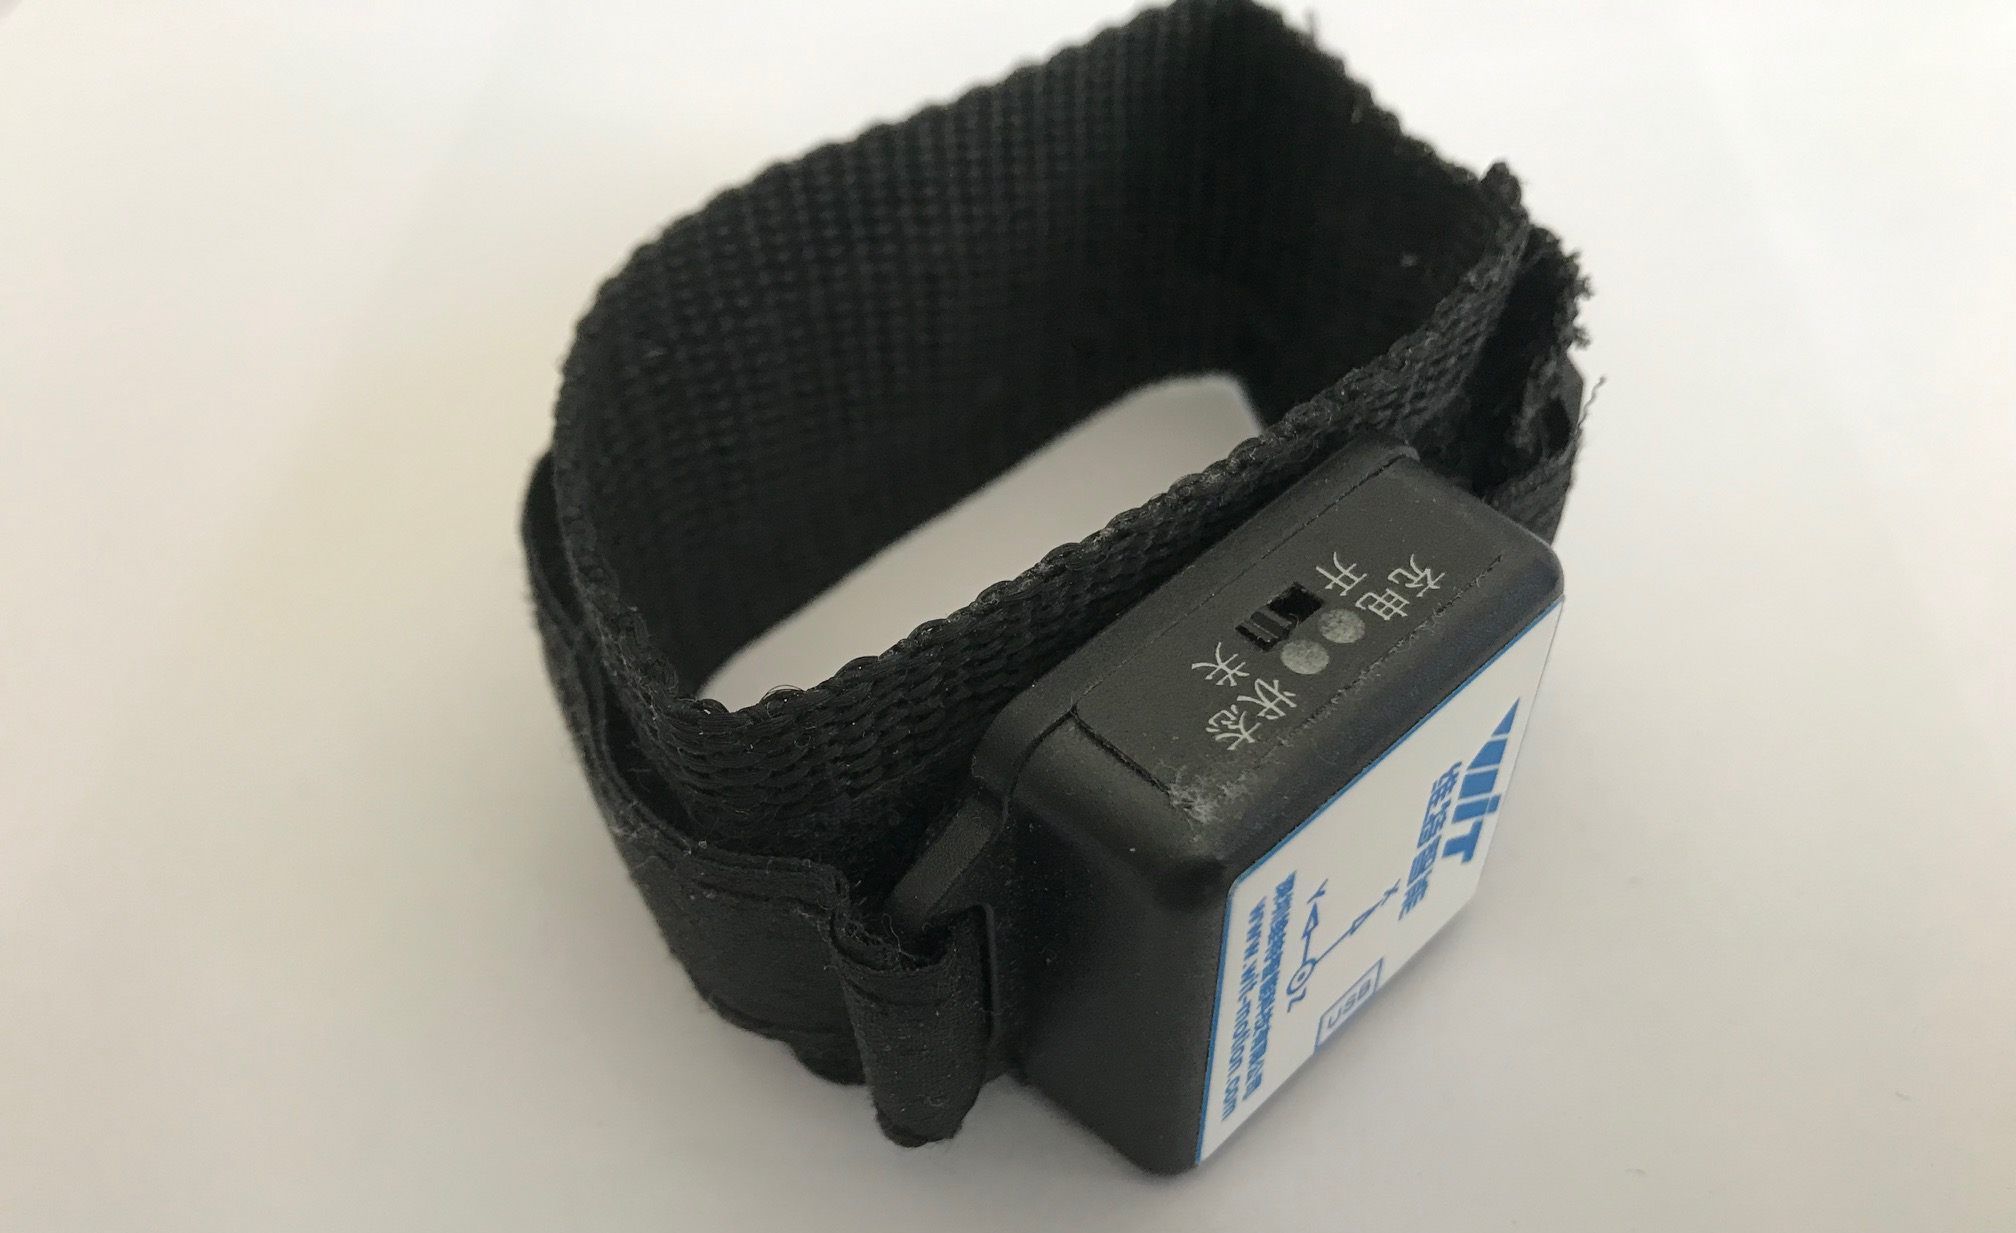
\includegraphics[width=.95\textwidth]{img/measuring_system/prototype.png}   
                        \end{minipage}};}
            \uncover<2->{\node[flowbox,fb-muted,right=of dev] (gui) {
                        \fbtitle{GUI}\vphantom{yÖ}
                        \nodepart{two}
                        \begin{minipage}{.29\textwidth}
                        \centering
                        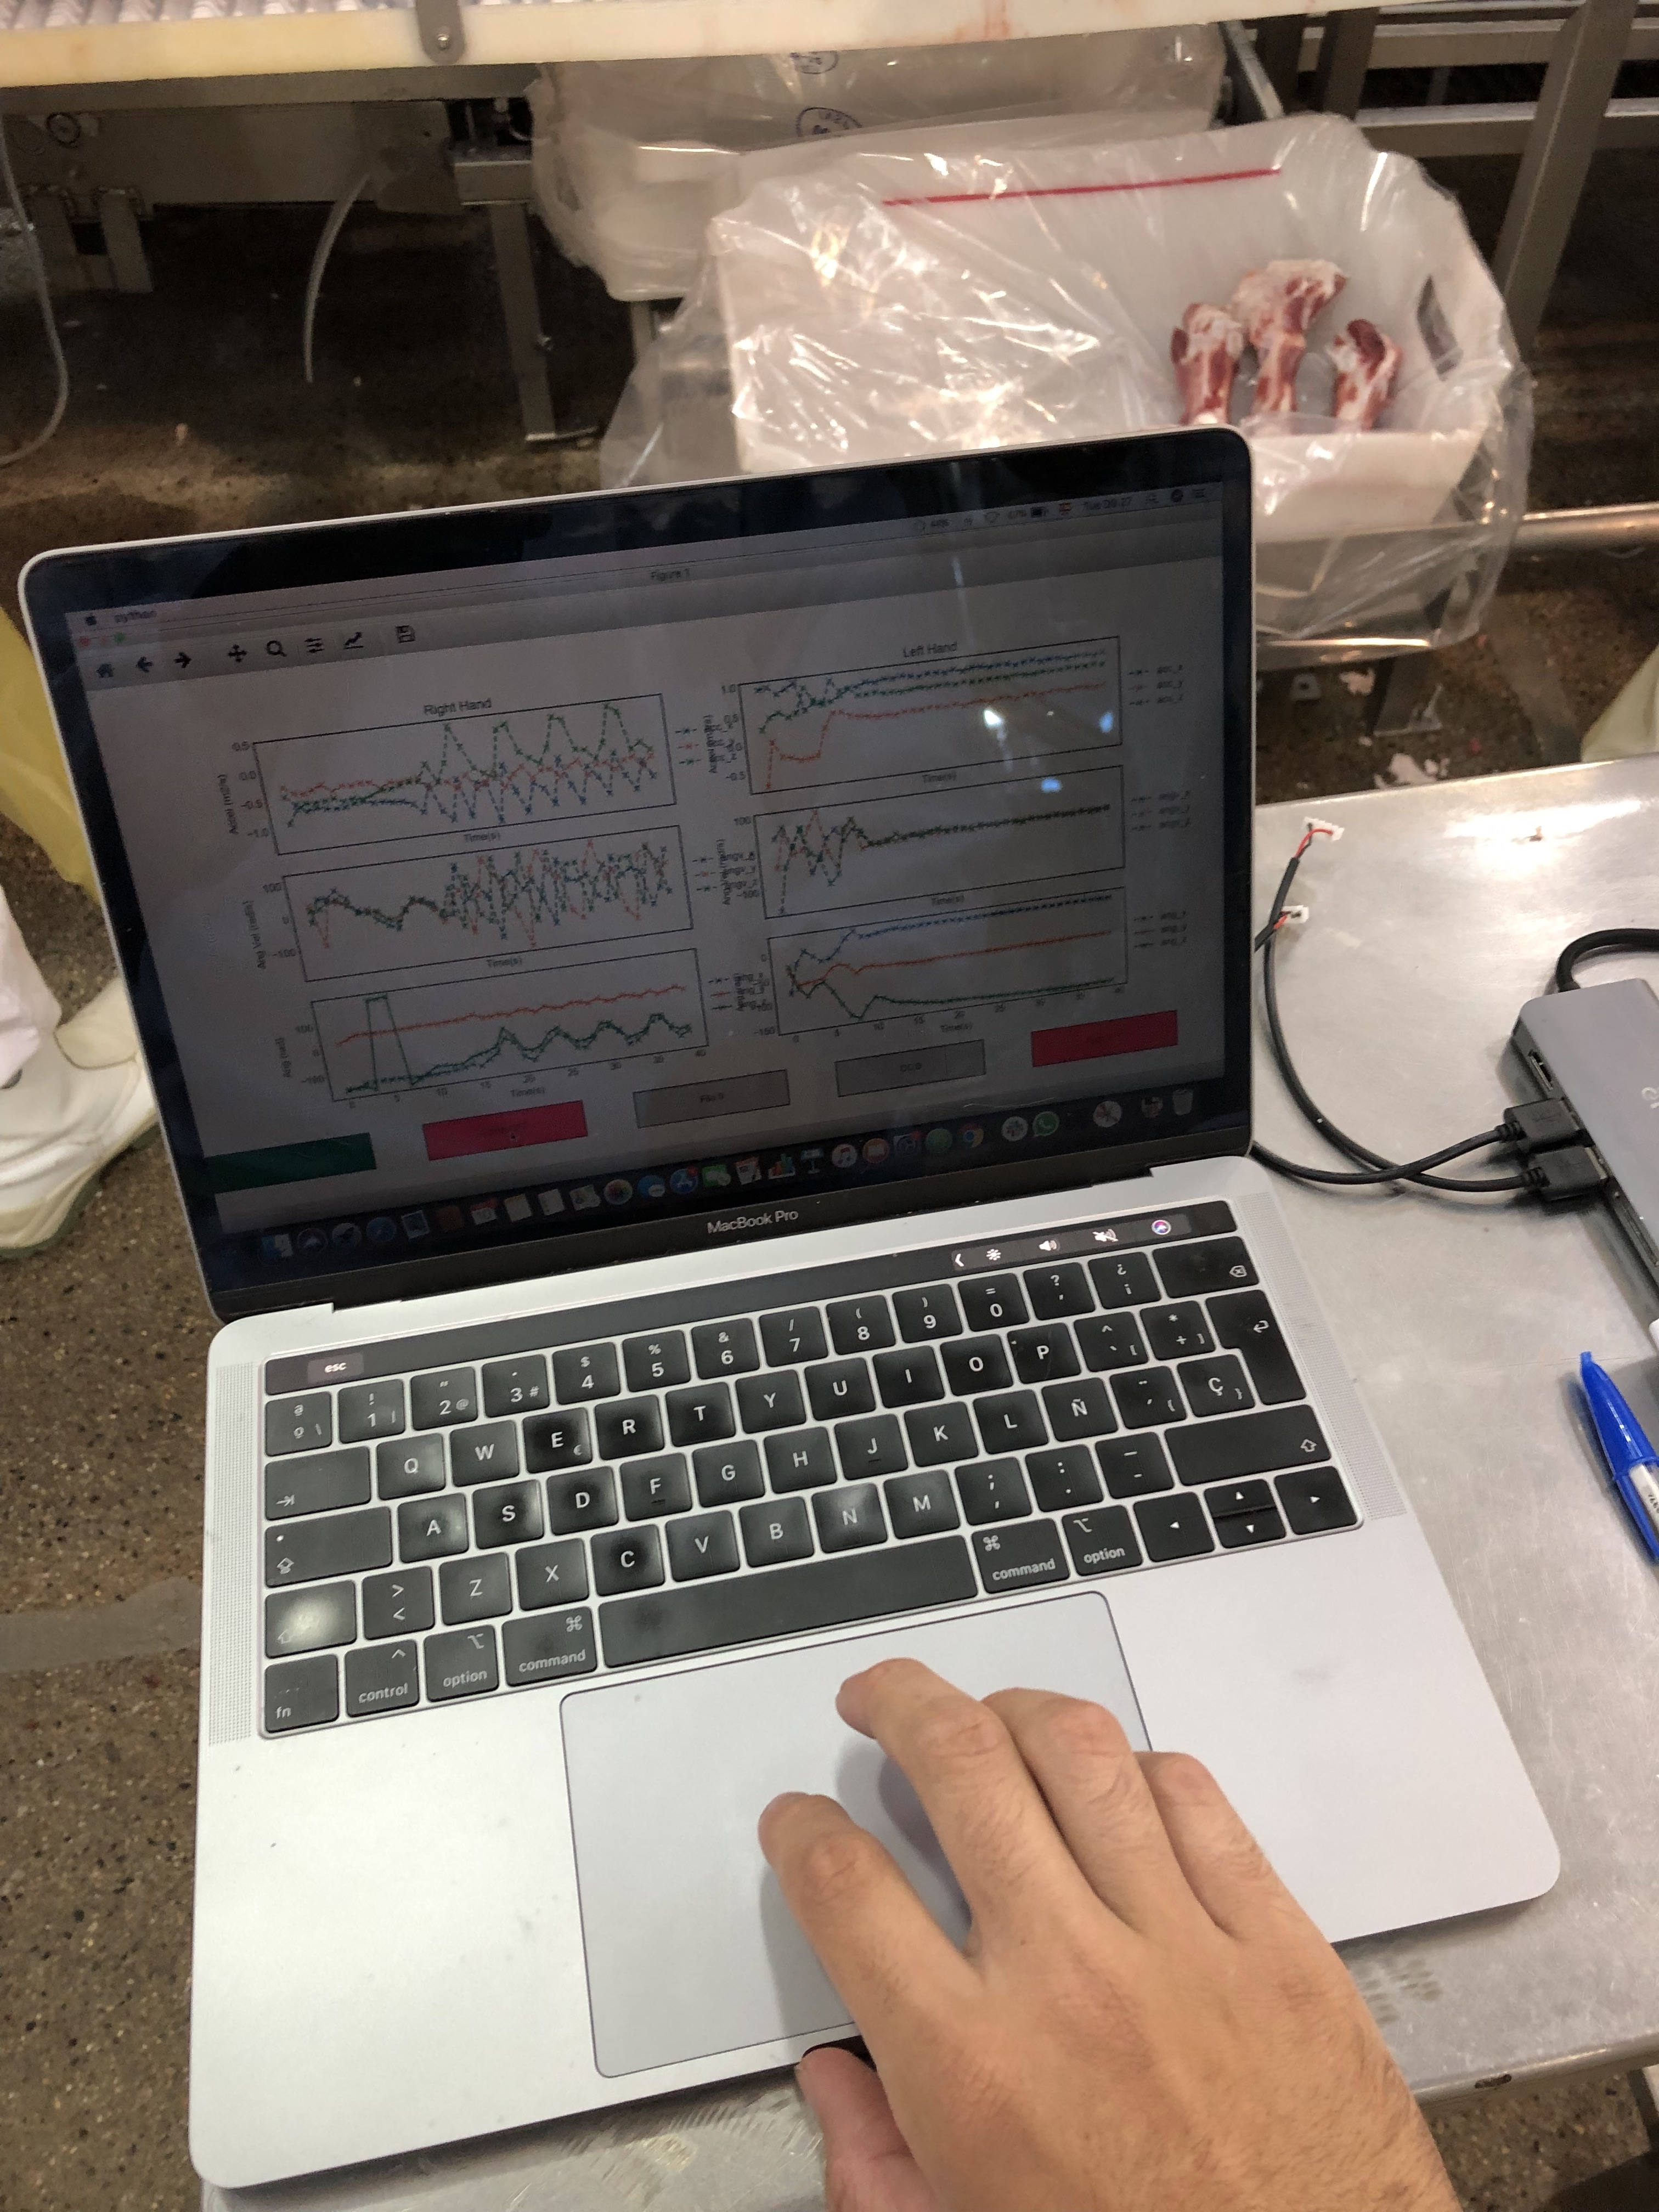
\includegraphics[width=.9\textwidth]{img/measuring_system/gui1.jpg}
                        \end{minipage}};
                        \draw[conn] (dev) -- (gui);}
            \uncover<3->{\node[flowbox,fb-muted,right=of gui] (data) {
                        \fbtitle{Batch Layer}\vphantom{yÖ}
                        \nodepart{two}
                        \begin{minipage}[t]{.2\textwidth}
                        \raggedright
                        \begin{itemize}
                        \item Innocuous
                        \item Indicator Evolution
                        \end{itemize}
                        \end{minipage}
                        \begin{minipage}[t]{.2\textwidth}
                        \raggedleft
                        \begin{itemize}
                        \item Task Extrapolation
                        \item Avoid Complexity
                        \end{itemize}
                        \end{minipage}};
                        \draw[conn] (gui) -- (data);}
        \end{tikzpicture}
    \end{center}
\end{frame}

% \begin{frame}{Prototype}
%     \begin{alertblock}{Components}
%         The prototype had 3 components.
%         \begin{enumerate}
%             \item The Graphical User Interface (GUI).
%             \item The wristband-based devices.
%             \item The Batch Layer.
%         \end{enumerate}
%     \end{alertblock}
% \end{frame}

\begin{frame}{Experiments}
\begin{alertblock}{Sample population}
    2 instructors and 18 Non-senior workers with varying degrees of experience.
\end{alertblock}    
\end{frame}



\begin{frame}{Experiments}
    \begin{alertblock}{Work tasks}
      Three work tasks. 
      \begin{enumerate}
          \item Instructor 1: Complete processing of the meat product
          \item Instructor 2: Femur and coxal deboning
          \item Non-senior workers: Femur deboning.
      \end{enumerate}
    \end{alertblock}
\end{frame}

\begin{frame}{Experiments}
    \begin{alertblock}{Assessment of WRMSDs}
        We propose a workflow for the assessment of WRMSDs based on the application of consecutive machine learning problems, using their predictions as input for a decision making rule.
    \end{alertblock}
\end{frame}